%This is a template for the University of Helsinki. If you have questions regarding the template please be in contact with uhbrand@helsinki.fi
%This template was designed by Zafar Hussain and Lalli Myllyaho for the Department of Computer Science, University of Helsinki.

% Compile with XeLaTeX or LuaLaTeX (e.g. latexmk -xelatex main.tex)
\documentclass[final]{beamer}
\mode<presentation>

\usepackage[english]{babel}
\usefonttheme{serif}
\usepackage{booktabs}
\usepackage{caption}
\usepackage[nolinks]{qrcode}
\usepackage{etoolbox}
% extra vertical space between list items
\AtBeginEnvironment{itemize}{\addtolength{\itemsep}{0.4ex}}

\usepackage[orientation=portrait,size=a0,scale=1.0]{beamerposter}
\usetheme[COM, twocolumn]{HYposter}
% Column width; the gutter between columns is set by \guttercolumn below
\renewcommand{\insertcolumnwidth}{0.45\paperwidth}

\addbibresource{bibliography.bib}

% Title and author info (from the GCB abstract)
\titlestart{IsoQuant4: }% first words in faculty colour
\titleend{A universal toolkit\\ for long-read transcriptomics}
\titlesize{\VeryHuge}

% \hfill separators: the headline stretches these lines across the page
\author{%
  \underline{Andrey Prjibelski}\textsuperscript{1}\hfill
  Lieke Michielsen\textsuperscript{2}\hfill
  Careen Foord\textsuperscript{2}\hfill
  Alexandru I. Tomescu\textsuperscript{1}\hfill
  Iman Hajirasouliha\textsuperscript{3}\hfill
  Hagen U. Tilgner\textsuperscript{2}\hfill
  \texttt{andrey.przhibelskiy@helsinki.fi}%
}
\institute{%
  \textsuperscript{1}Department of Computer Science, University of Helsinki, Finland\hfill
  \textsuperscript{2}Feil Family Brain and Mind Research Institute, Weill Cornell Medicine, NY, USA\hfill
  \textsuperscript{3}Institute for Computational Biomedicine, Weill Cornell Medicine, NY, USA%
}

% Smaller captions than the theme default
\captionsetup{font={footnotesize},textfont={bf},aboveskip=12pt,belowskip=2pt}
\renewcommand\bibfont{\tiny}

% Calibri to match the figures; Carlito is its metric-compatible clone
\IfFontExistsTF{Calibri}{\setmainfont{Calibri}}{\setmainfont{Carlito}}
\IfFontExistsTF{Calibri}{\setsansfont{Calibri}}{\setsansfont{Carlito}}
% Conference guidelines: >=0.8cm text with >=1.1cm line spacing
\linespread{1.12}

\begin{document}

\begin{poster}

% ============================ LEFT COLUMN ============================
\newcolumn

\section{Introduction}
\justifying
Single-cell and spatial transcriptomics combined with long-read sequencing
enable isoform-level profiling and the study of alternative splicing.
We present \textbf{IsoQuant4} --- a universal toolkit for processing
long-read RNA-seq data, \textbf{Spl-IsoFind} --- a package for discovering spatially variable isoforms and their application to mouse brain data.

\section{IsoQuant4 features}
\justifying
\begin{itemize}
  \item Feature quantification 
  \begin{itemize}
        \item Genes/transcripts
        \item Exons/splice junctions/intron retentions
        \item Works for bulk, single-cell and spatial data
  \end{itemize}
  \item Reference-based and \textit{de novo} transcript discovery
  \item Barcode calling:
  \begin{itemize}
        \item 10x single-cell v2/v3/v4
        \item 10x Visium/VisiumHD
        \item Curio
        \item Stereo-seq
        \item cDNA de-concatenation
  \end{itemize}
  \item Universal barcode calling for any custom protocol
  \item PCR deduplication;
  \item Poly(A) site and TSS detection
  \item Fusion gene discovery
\end{itemize}

\section{IsoQuant4 pipeline}
\justifying
\begin{figure}
    \hspace*{-2cm}% adjust to shift the figure left/right
    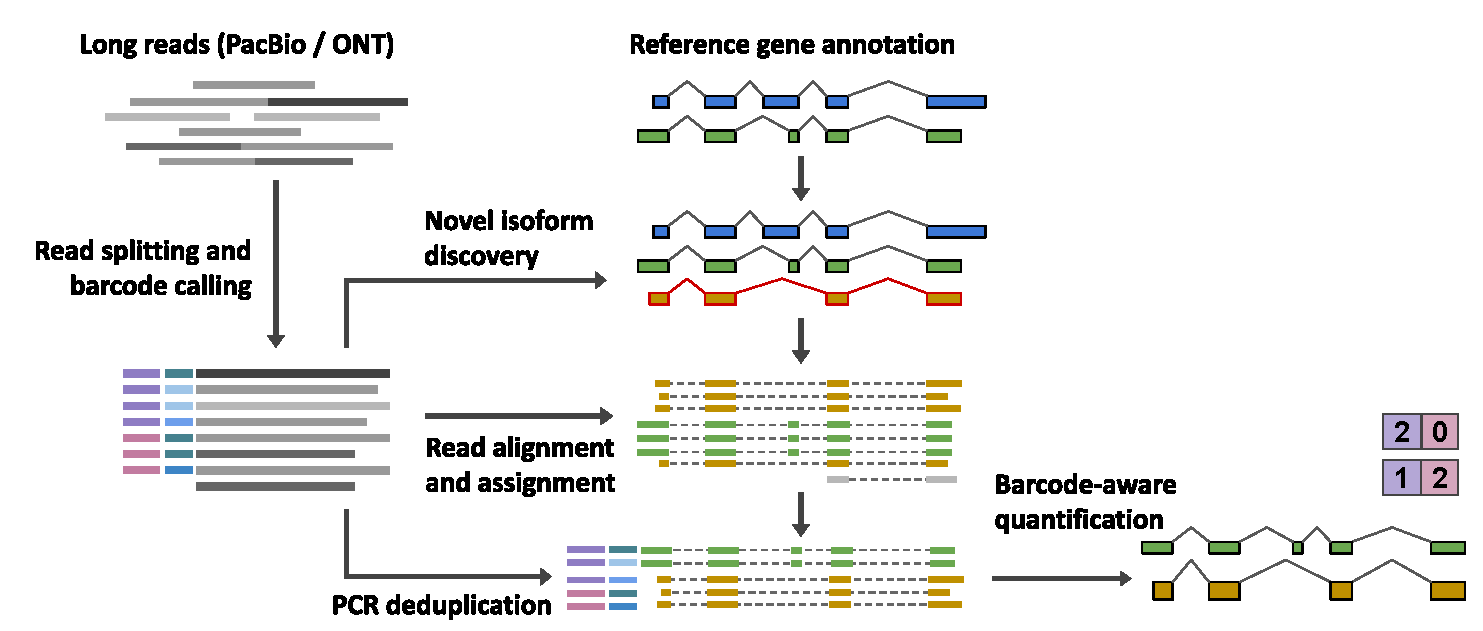
\includegraphics[width=1.0\textwidth]{figures/pipeline.pdf}
    \label{fig:pipeline}
\end{figure}

\section{Barcode calling}
\justifying
\begin{figure}
    \hspace*{-1cm}% adjust to shift the figure left/right
    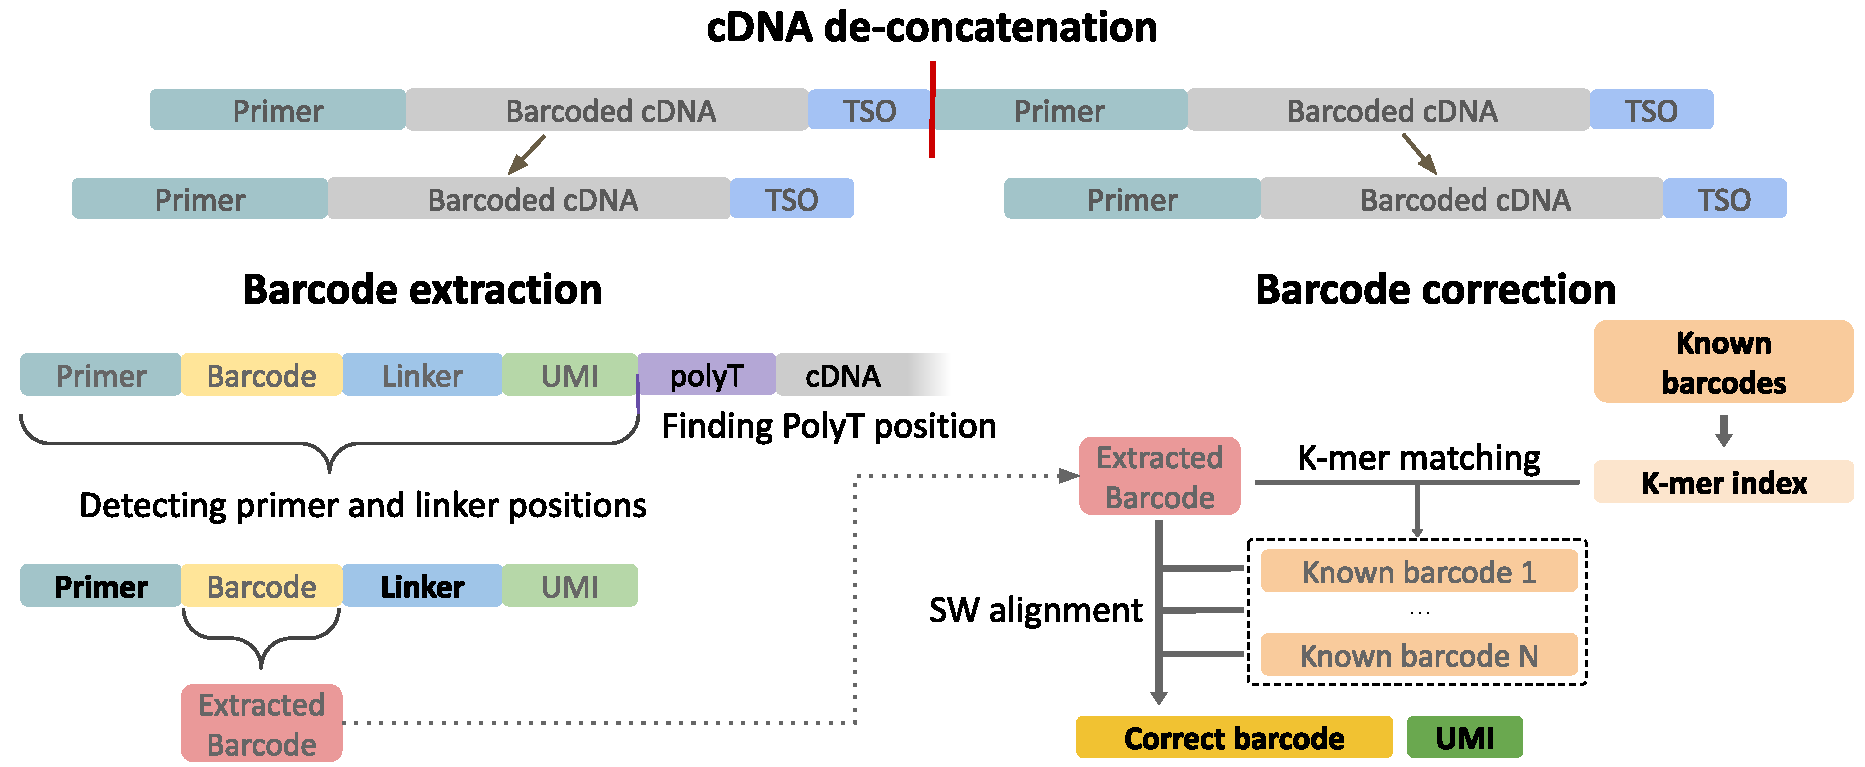
\includegraphics[width=1.0\textwidth]{figures/barcode_calling.pdf}
    \label{fig:barcode}
\end{figure}

\section{Scaling to 500M barcodes}
\justifying
\begin{minipage}[c]{0.42\textwidth}
\begin{table}
    \begin{tabular*}{0.92\textwidth}{@{\extracolsep{\fill}} l r }
    \toprule
        \textbf{Protocol} & \textbf{Cells/spots} \\
    \midrule
        10x single-cell & 10K \\
        Curio           & 100K \\
        10x Visium HD   & 10M \\
        Stereo-seq      & \textbf{500M} \\
    \bottomrule
    \end{tabular*}
\end{table}
\end{minipage}%
\begin{minipage}[c]{0.57\textwidth}
\begin{itemize}
  \item \textbf{Barcode indexing:} 500M barcodes indexed in 10 minutes;
  \item \textbf{Read processing:} 60M reads/h (10M reads/h with
        de-concatenation).
\end{itemize}
\end{minipage}

\section{Barcode detection accuracy}
\justifying
Simulated ONT reads, 3.8\% error rate, 25\,bp barcodes (left); on Visium
HD, IsoQuant4 yields 2.5--3.4$\times$ fewer false positives (right).

\vspace{0.5em}
\begin{minipage}[t]{0.44\textwidth}
\footnotesize
\begin{table}
    \begin{tabular*}{\textwidth}{@{\extracolsep{\fill}} l r r }
    \toprule
        \textbf{Simulated} & \textbf{1 cDNA} & \textbf{Concat.} \\
        \textbf{ONT}       & \textbf{/read}  & \textbf{cDNAs} \\
    \midrule
        Precision & \textbf{99.95\%} & \textbf{99.94\%} \\
        Recall    & 76.62\% & 78.07\% \\
    \bottomrule
    \end{tabular*}
\end{table}
\end{minipage}\hfill
\begin{minipage}[t]{0.54\textwidth}
\footnotesize
\begin{table}
    \begin{tabular*}{\textwidth}{@{\extracolsep{\fill}} l l r r }
    \toprule
        \textbf{Visium HD} & & \textbf{IsoQuant4} & \textbf{SpaceRanger} \\
    \midrule
        2\,\textmu m & Precision & \textbf{97.58\%} & 94.18\% \\
                     & Recall    & 76.08\% & 78.88\% \\
        8\,\textmu m & Precision & \textbf{99.29\%} & 97.50\% \\
                     & Recall    & 76.39\% & 79.45\% \\
    \bottomrule
    \end{tabular*}
\end{table}
\end{minipage}

% QR codes
\vspace{0.5em}
\begin{center}
\begin{minipage}[t]{0.30\textwidth}\centering
    \qrcode[height=4.5cm]{https://github.com/ablab/IsoQuant}\\[1.5ex]
    {\footnotesize\bfseries IsoQuant}
\end{minipage}\hfill
\begin{minipage}[t]{0.30\textwidth}\centering
    \qrcode[height=4.5cm]{https://github.com/tilgnerlab/Spl-IsoFind}\\[1.5ex]
    {\footnotesize\bfseries Spl-IsoFind}
\end{minipage}\hfill
\begin{minipage}[t]{0.30\textwidth}\centering
    \qrcode[height=4.5cm]{https://doi.org/10.1038/s41592-026-03211-w}\\[1.5ex]
    {\footnotesize\bfseries Nature Methods paper}
\end{minipage}
\end{center}

% ============================ RIGHT COLUMN ===========================
\guttercolumn
\newcolumn

\section{Spatial isoform variability}
\begin{figure}
    \centering
    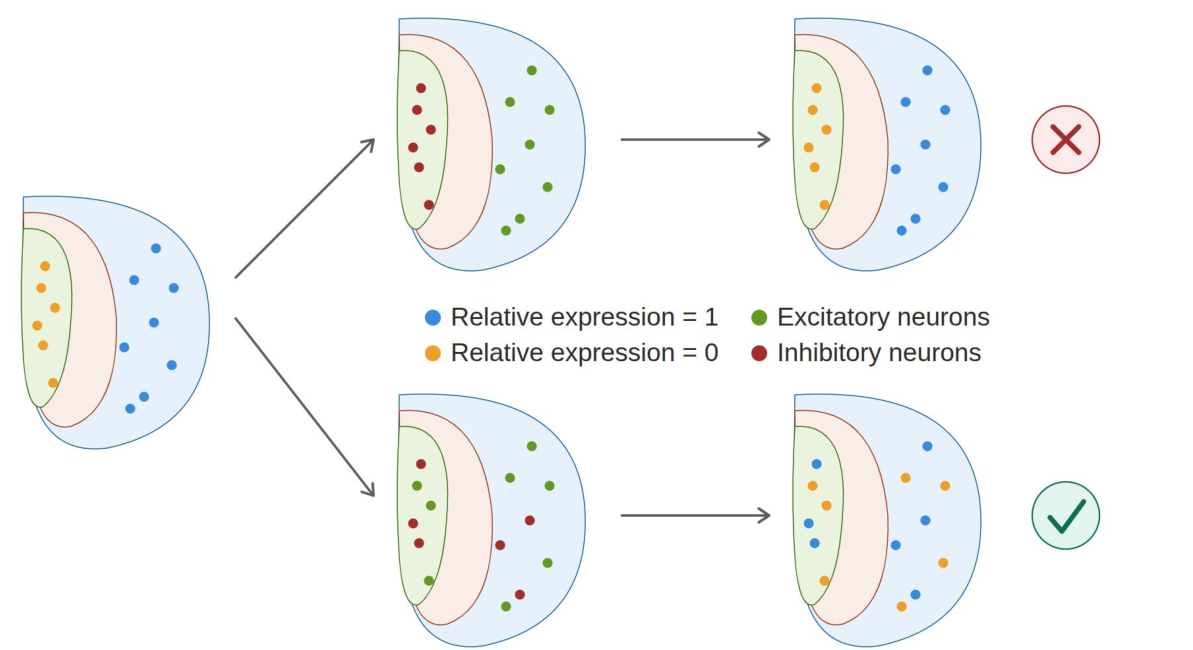
\includegraphics[width=1.0\textwidth]{figures/variability.pdf}
    \label{fig:variability}
\end{figure}

\section{Spl-IsoFind}
\justifying
Spl-IsoFind detects spatially variable isoforms linked to and not linked to pre-defined brain regions.
The latter is detected via Moran's~$I$ spatial autocorrelation and permutation tests.
\begin{figure}
    \centering
    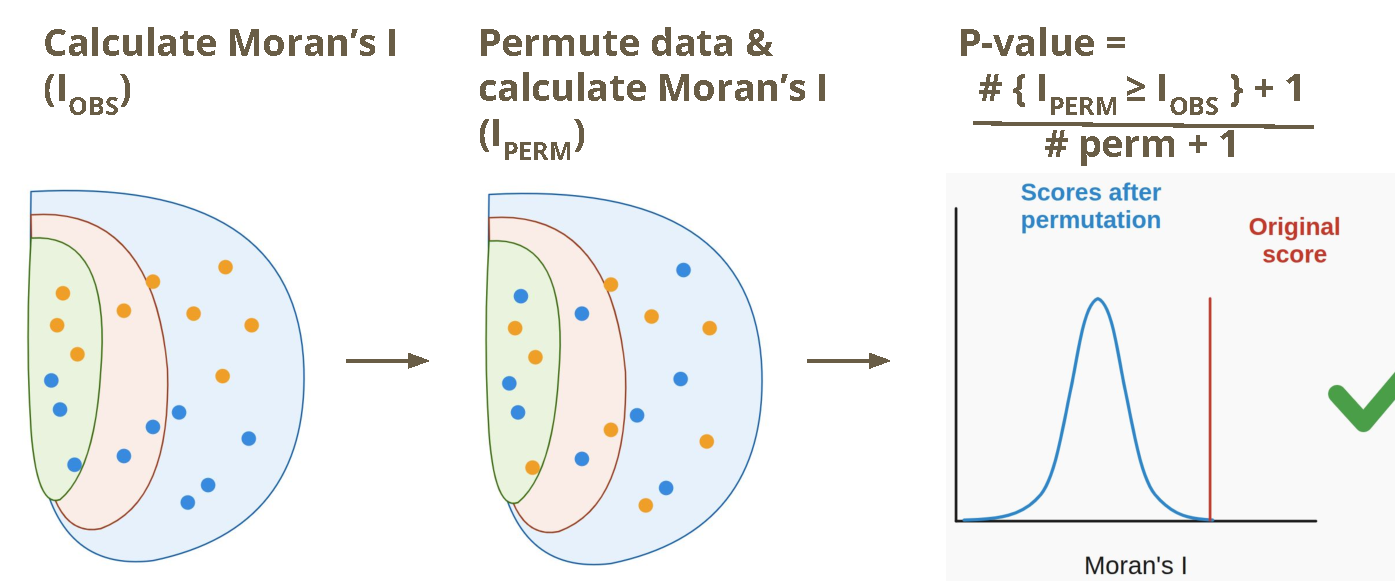
\includegraphics[width=0.9\textwidth]{figures/splisofind.pdf}
    \label{fig:splisofind}
\end{figure}

\section{Results: mouse brain}
\justifying
Applied to mouse brain spatial long-read data with nanometer resolution, our
toolkit discovers spatially variable isoforms at single-cell level,
reproducibly across platforms and protocols.
\begin{figure}
    \centering
    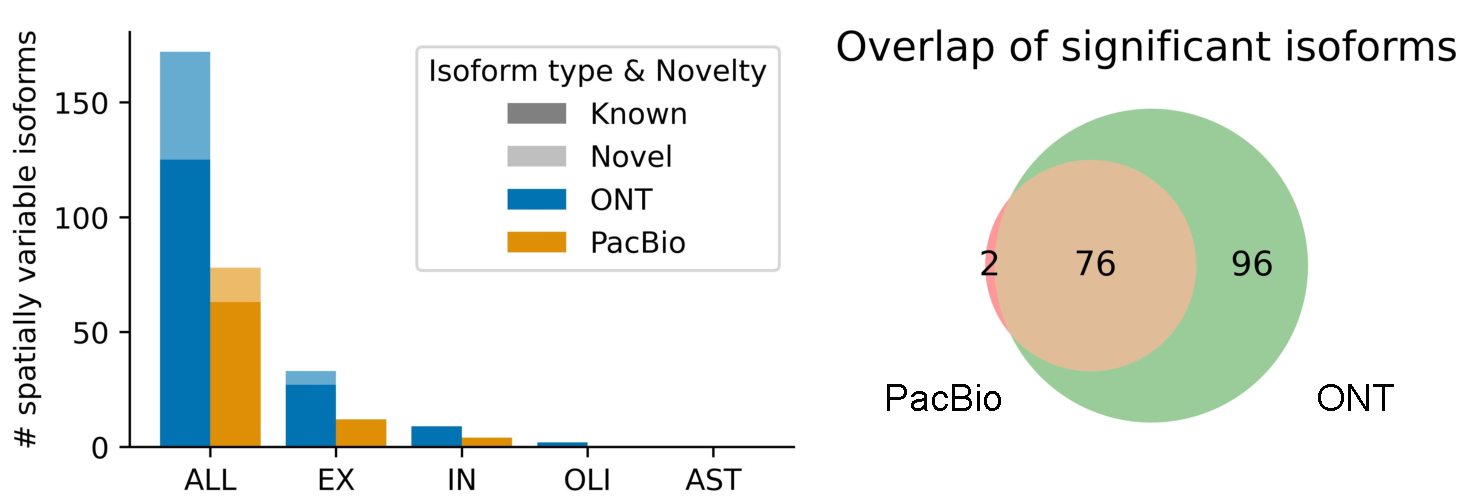
\includegraphics[width=0.67\textwidth]{figures/sv_isoforms.pdf}
    \caption{\sffamily Spatially variable isoforms per cell type (left) and
    PacBio/ONT overlap (right).}
    \label{fig:svisoforms}
\end{figure}

\begin{figure}
    \centering
    \begin{minipage}[c]{0.46\textwidth}
        \centering
        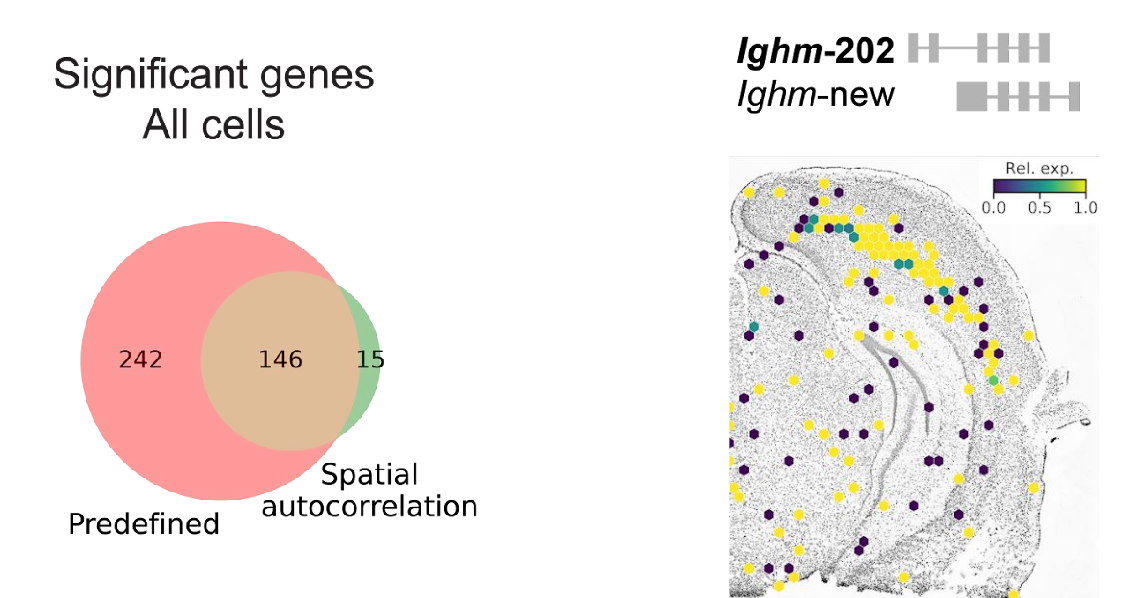
\includegraphics[width=\textwidth]{figures/sv_genes_ighm.pdf}
    \end{minipage}\hfill
    \begin{minipage}[c]{0.32\textwidth}
        \centering
        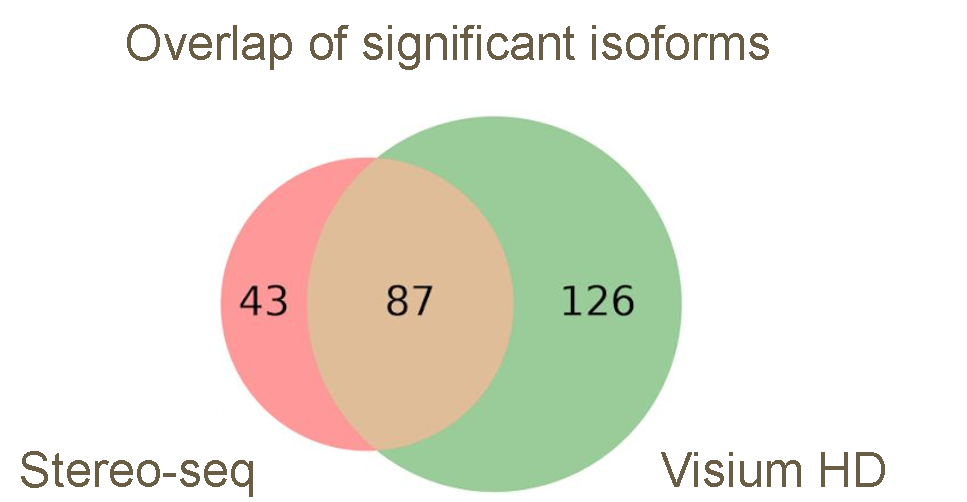
\includegraphics[width=0.92\textwidth]{figures/protocol_overlap.pdf}
    \end{minipage}
    \caption{\sffamily Predefined regions vs.\ spatial autocorrelation; a
    novel \textit{Ighm} isoform; Stereo-seq/Visium HD overlap.}
    \label{fig:ighm}
\end{figure}

\section{Conclusions}
\justifying
\begin{itemize}
  \item First long-read spatial isoform mapping at single-cell resolution;
  \item Long-read sequencing combined with Stereo-seq and 10x Visium HD;
  \item Universal pipeline for bulk, single-cell and spatial long-read data;
  \item Spl-IsoFind detects spatially variable isoforms;
  \item Cell-type-specific spatially variable isoforms in adult mouse brain.
\end{itemize}

\section{Acknowledgements}
\justifying
\footnotesize
% TODO: fill in grant acknowledgements below
[GRANT ACKNOWLEDGEMENTS PLACEHOLDER --- funding agencies and grant numbers]

This poster was formatted and compiled using Claude AI. \\

Software: \texttt{github.com/ablab/IsoQuant} \quad
\texttt{github.com/tilgnerlab/Spl-IsoFind}

\vspace{0.5em}
\printbibliography[heading=none]

\end{poster}
\end{document}
